\documentclass[onlytextwidth]{beamer}
\usepackage[utf8]{inputenc}
\usepackage{microtype}
\usepackage{amsmath}
\usepackage{amssymb}
\usepackage[nomessages]{fp} %\FPeval{\var-name}{2*sin(pi/6)}
\usepackage{siunitx} %units in math. eg 20\milli\meter
\usepackage{yhmath} % for arcs, overparenth command
\usepackage{tikz} %graphics
\usetikzlibrary{quotes, angles}
%\usepackage{graphicx} already loaded by beamer class
%consider setting \graphicspath{{images/}}
%\parskip ?? to avoid paragraph indent
\usepackage{multicol} %may not need this package, just columns environment
\usepackage{venndiagram}

\subtitle[BECA]{Bronx Early College Academy}
\author[Huson]{Christopher J. Huson PhD}

\setbeamertemplate{headline}{\vskip2mm 
  BECA / \insertshortauthor \, / \inserttitle
  \hfill 
  \insertsection
  }

\title{Routines and Expectations}
\date{2022-2023}

\begin{document}
\frame{\titlepage}

%\section[Outline]{}
%\frame{\tableofcontents}

\section{0.1 Personal tools every day \hfill 8 September}
\begin{frame}{Begin class on time}
  {Welcome back to school \hfill \alert{0.1 Thursday 8 September}}
  \begin{block}{Expectation: On your desk, every day, start of class}
  \begin{enumerate}
      \item Notebook, pencil/pen
      \item Pocket folder (for worksheets)
      \item Tools: calculator, ruler, Chromebook (charged)
  \end{enumerate}
  \end{block}
  Supply list: Composition book, folder, looseleaf, pencils \& pens, \\*
  ruler, calculator
  \end{frame}

\begin{frame}{Take class notes in a composition book}
  \begin{block}{Use this notebook format (required)}
    \begin{enumerate}
      \item Outside cover: ``Geometry'', your first and last name
      \item First page: your name, my contact info, your passwords \\
      \qquad Dr. Huson / chuson@schools.nyc.gov / 917-648-5632 \vspace{0.25cm}
      \item Each page in the top left corner: \\
      \emph{I can measure and diagram my world} \hfill 8 September 2022 \vspace{0.25cm}
      \item Copy definitions using your own words
      \item Write down example diagrams and problems
    \end{enumerate}
    \end{block}
  \end{frame}

\section{0.2 Casio calculator \hfill 8 September}
\begin{frame}{Casio fx-9750GIII calculator (due Friday 16 September)}
  \begin{columns}
    \column{0.4\textwidth}
      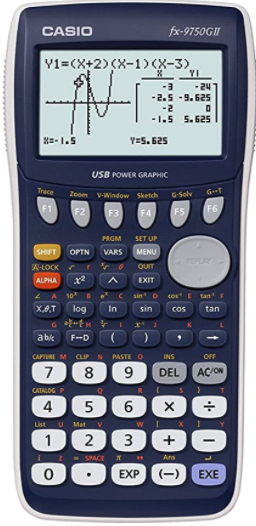
\includegraphics[width=2.75cm]{../graphics/casio_fx-9750GII.png}
    \column{0.6\textwidth}
      In the high school at BECA we use the Casio fx-9750GIII.\\[5pt] 
      It is allowed on the Regents exams, SAT tests, and International Baccalaureate exams.\\[5pt]
      The older model is also acceptable, Casio fx-9750\alert{GII}.\\[5pt]
      (see me if buying a calculator is a hardship for your family)
    \end{columns} \vspace{1cm}
  Supply list: Composition book, folder, looseleaf paper, pencils \& pens, ruler, calculator
\end{frame}

\section{0.3 Dismissal \hfill 8 September}
\begin{frame}{End-of-class cleanup begins 3 minutes before the bell}
  \begin{block}{Work until told to begin dismissal routine}
    \begin{enumerate}
      \item Classwork goes in folder (complete at home)
      \item Put homework in folder
      \item Return desks (if necessary)
      \item Check for garbage, remind yourself to push in your chair
      \item Stay seated and quiet until dismissed by teacher
    \end{enumerate}
    \end{block}
  \end{frame}

\end{document}